In this section we discuss the results of classification and error recognition of actions in table tennis. We trained an HMM for forehand, backhand, and serve actions using 10 samples in each dataset. Figure \ref{fig-viterbi} shows the 6 acceleration and rotation features and the most likely state sequence of each action using a sample in our test data.

By looking at the most likely hidden sequences we can tell that the classifiers divided the actions into 4 parts, where the beginning part is when the hand starts from rest. The second part is the preparation phase where the racket goes slightly back to prepare for hitting the ball. The third part is when it is moving towards the ball and the fourth part is when the hand goes back to rest. As we can see, the preparation phase in forehand and serve is longer than backhand. The reason is because in the backhand gesture the hand does not have enough space to prepare for hitting the ball, while in forehand and serve we have much more space.

Table \ref{table-score} shows the F1 score of recognizing the three gestures. Using the entire length of gestures for classification resulted in perfect classification. Using a sliding window also we had perfect recognition of the backhand and about $90\%$ accuracy in recognizing forehand and serve actions.

In a different experiment we also included the threshold HMM in the classifier to identify non-action parts. Table \ref{table-scoreThresh} shows the precision, recall, and F1 score of this test. As you can see, the precision of recognizing backhand and serve is 1, but for forehand and non-action gestures we received about $80\%$ precision. On the other hand the recall rate for non-action movement is 1. With this information we can tell that the classifier can perfectly recognize all the transition parts, but it sometimes classifies a non-action movement as forehand. 

One problem novice players have when starting table tennis is with the serve action. To have a good serve one should control the movement of the wrist and prevent it from bending. We collected examples of bending the hand when serving and experimented to see if we can recognize this error with DTW. Figure \ref{fig-distance} shows the distance matrix and the corresponding frames between a bad sample of the serve action and the good sample in our dataset. Also figure \ref{fig-good-bad} shows the comparison of the error rate of a bad sample and a good sample. As you can see on the bad serve sample, we get a very high error when the player hits the ball because of bending of the wrist. 

\begin{figure}
\centering
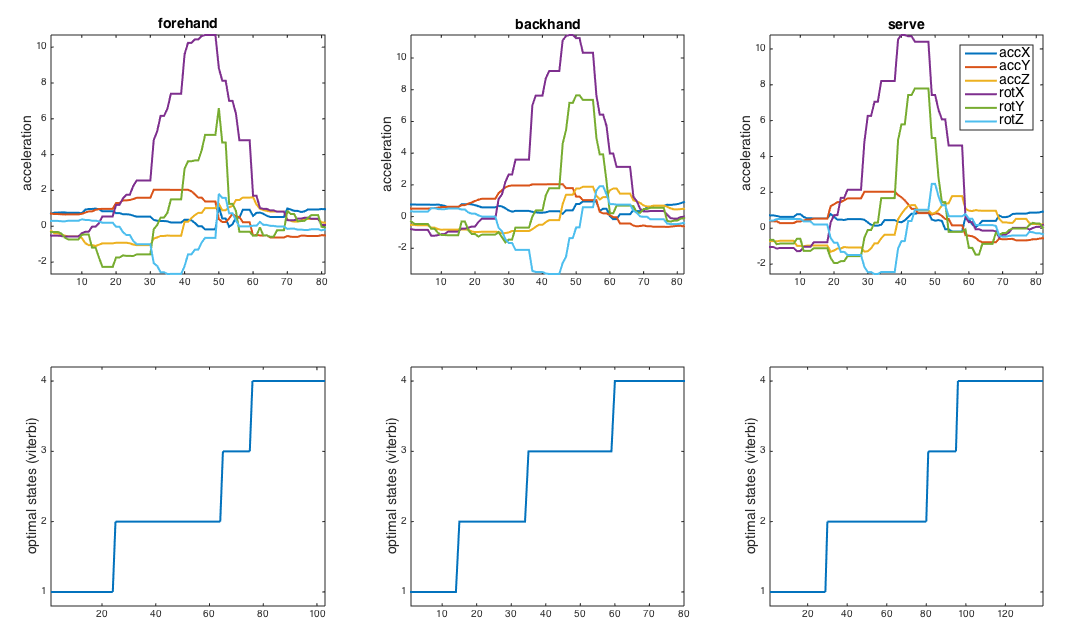
\includegraphics[width=3in]{resources/viterbi.png}
\caption{Most likely state sequence of a serve test action using Viterbi}
\label{fig-viterbi}
\end{figure}
\begin{table}[h]
\begin{tabular}{cccc}
                                        & \cellcolor[HTML]{C0C0C0}Forehand & \cellcolor[HTML]{C0C0C0}Backhand & \cellcolor[HTML]{C0C0C0}Serve \\
\cellcolor[HTML]{C0C0C0}entire sequence & 1.00                             & 1.00                             & 1.00                          \\
\cellcolor[HTML]{C0C0C0}window size 16  & 0.86                             & 0.89                             & 0.84                          \\
\cellcolor[HTML]{C0C0C0}window size 32  & 0.91                             & 1.00                             & 0.93                         
\end{tabular}
\caption{F1 score for recognizing each action using the whole gesture and sliding window of size 16 and 32 frames}
\label{table-score}
\end{table}
\begin{table}[h]
\begin{tabular}{ccccc}
                                  & \cellcolor[HTML]{C0C0C0}Forehand & \cellcolor[HTML]{C0C0C0}Backhand & \cellcolor[HTML]{C0C0C0}Serve & \cellcolor[HTML]{C0C0C0}Non-Gesture \\
\cellcolor[HTML]{C0C0C0}Precision & 0.84                             & 1.00                             & 1.00                          & 0.86                                \\
\cellcolor[HTML]{C0C0C0}Recall    & 0.92                             & 0.77                             & 0.78                          & 1.00                                \\
\cellcolor[HTML]{C0C0C0}F1 score  & 0.88                             & 0.87                             & 0.87                          & 0.92                               
\end{tabular}
\caption{Recognizing ping pong gestures from transition parts using a sliding window of size 32}
\label{table-scoreThresh}
\end{table}
\begin{figure}[tbp]
	\centering
	\subfloat[Good Serve]{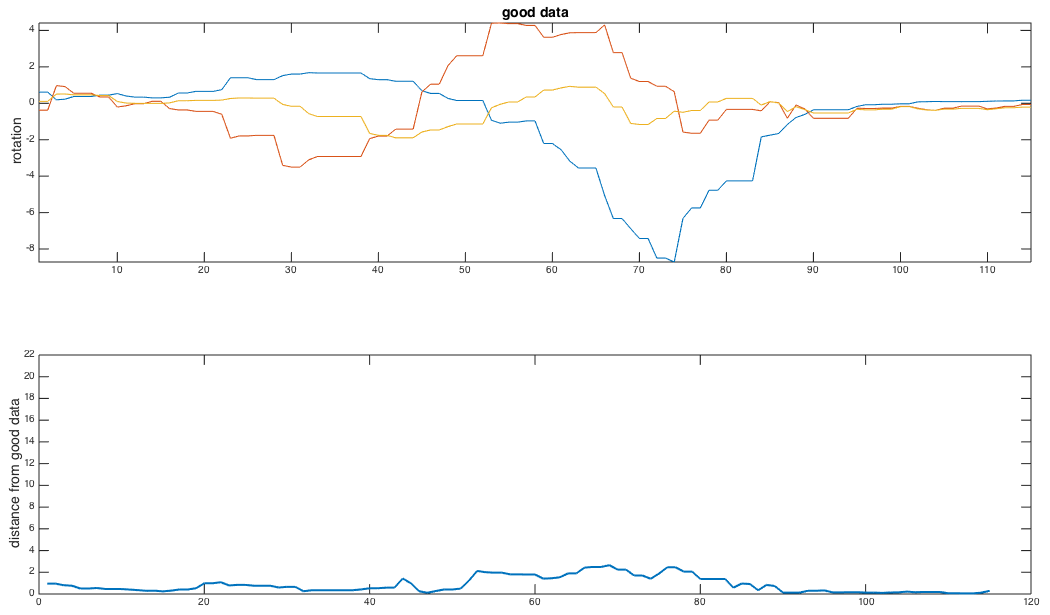
\includegraphics[width=3in]{resources/good.png}}\quad
	\subfloat[Bad Serve]{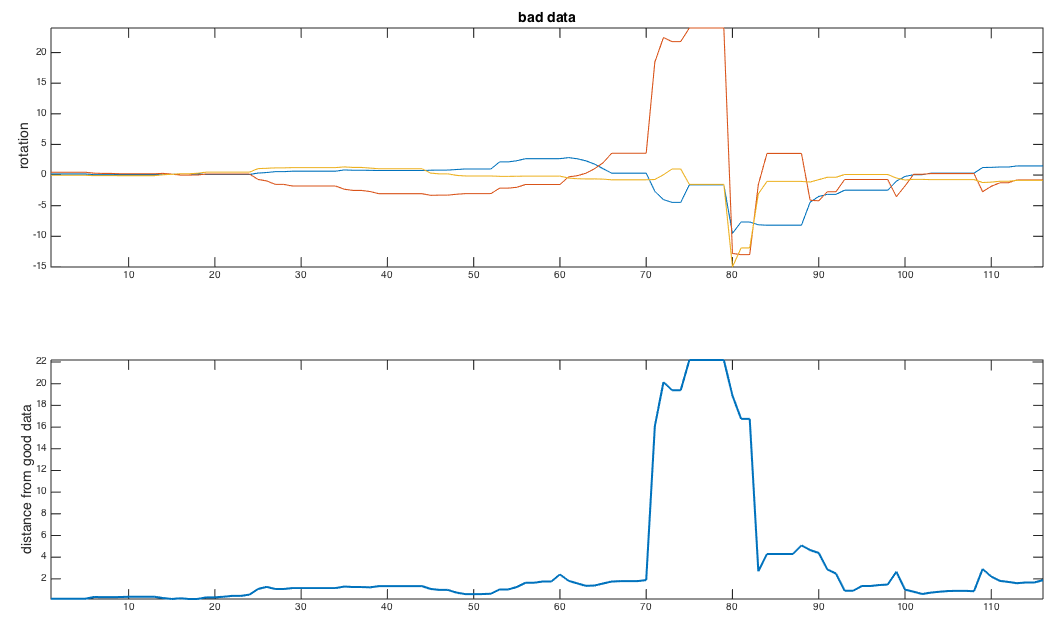
\includegraphics[width=3in]{resources/bad.png}}\\	
	\caption{3D rotation and error rate of a good and bad serve computed with DTW}
    \label{fig-good-bad}
\end{figure}
\begin{figure}
\centering
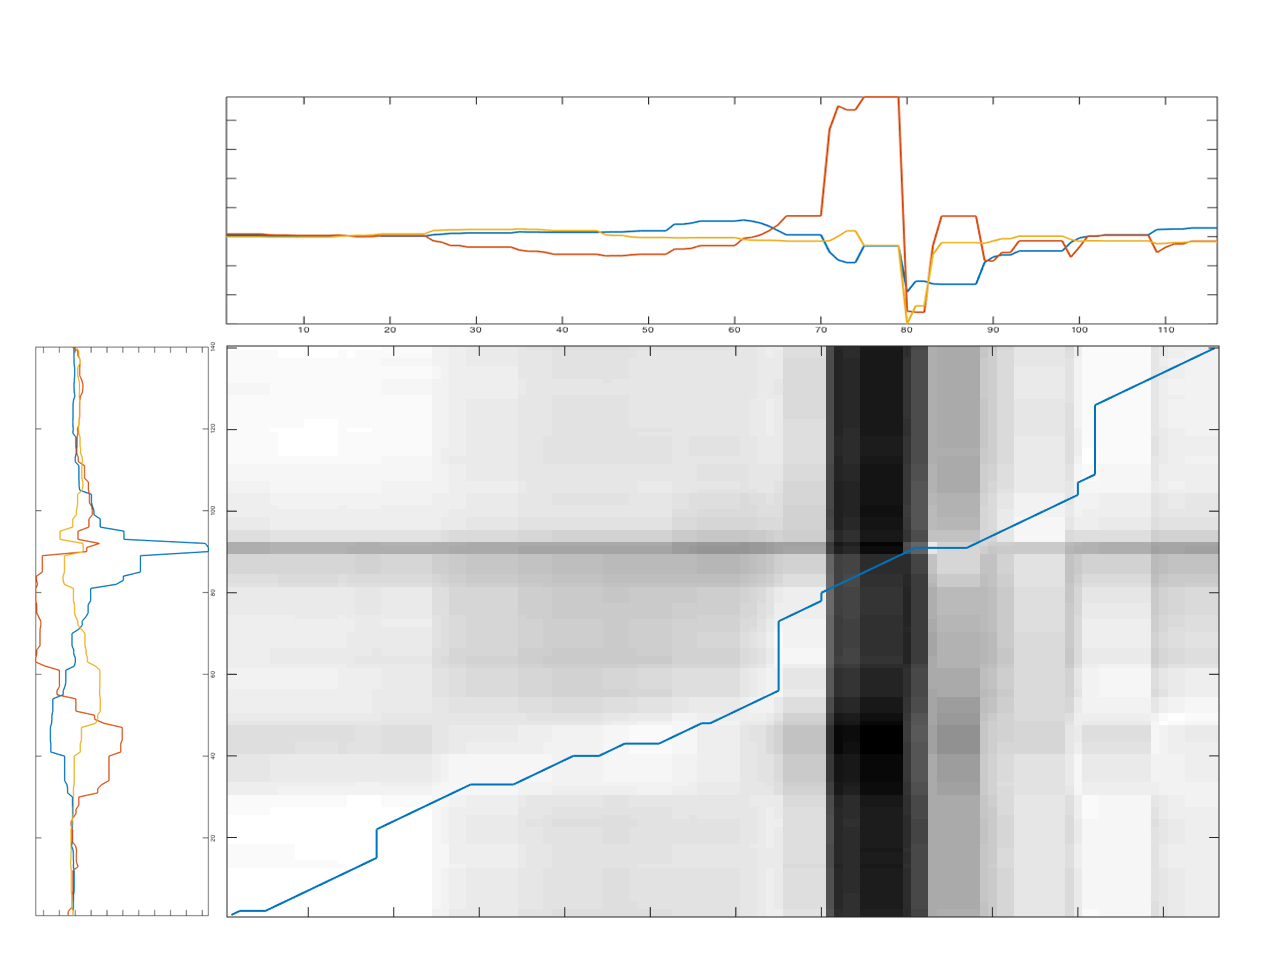
\includegraphics[width=3in]{resources/distance.jpg}
\caption{Distance between the 3 axes rotation of a good and bad serve}
\label{fig-distance}
\end{figure}
